\documentclass[../Cours.tex]{subfiles}
\begin{document}

\chapitre{Parallélogramme}

\partie{Nomenclature des parallélogrammes}

\begin{center}
    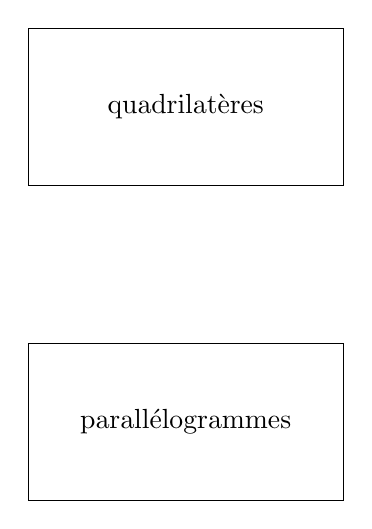
\begin{tikzpicture}
        \draw (-2,10) rectangle (2,12);
        \node at (0,11) {quadrilatères};
        \draw (-2,6) rectangle (2,8);
        \node at (0,7) {parallélogrammes};
    \end{tikzpicture}
\end{center}

\souspartie{Losange}
\definition{Un losange est un parallélogramme qui a 4 côtés égaux.}
\illustration{}
\propriete{Dans un losange, les diagonales sont perpendiculaires.}

\souspartie{Rectangle}
\definition{Un rectangle est un parallélogrammes dont tous les angles sont égaux à \ang{90}.}
\illustration{}
\propriete{Dans un rectangle, les diagones sont de même longueur.}

\souspartie{Carré}
\definition{Un parallélogramme qui a les mêmes propriétés que le losange et le rectangle est un carré.}
\illustration{}


\clearpage
\EXERCICES
\begin{questions}
    \exercicetitre{}
\end{questions}

\end{document}